% Figure from MATH 493 notes, section 54 (internal direct sums). Added, not from lecture (after the board sketch of 10/26).
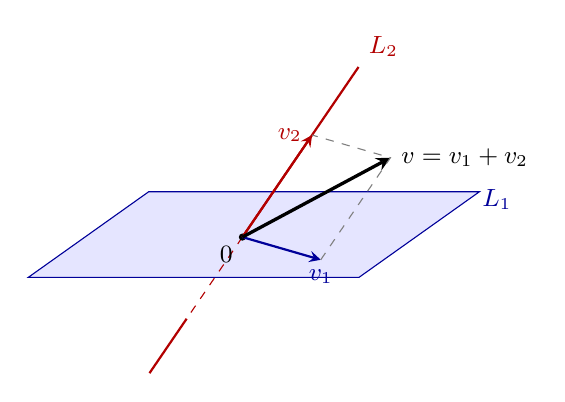
\begin{tikzpicture}[>=stealth, font=\small, x={(1cm,0cm)}, y={(0.45cm,0.32cm)}, z={(0cm,1cm)}]
    % plane L1 = span(e1, e2)
    \fill[blue!10] (-2,-1.6,0) -- (2.2,-1.6,0) -- (2.2,1.8,0) -- (-2,1.8,0) -- cycle;
    \draw[blue!60!black] (-2,-1.6,0) -- (2.2,-1.6,0) -- (2.2,1.8,0) -- (-2,1.8,0) -- cycle;
    \node[blue!60!black, anchor=west] at (2.25,1.5,0) {$L_1$};
    % line L2 = span(1, 0.4, 1.6), drawn through the origin (hidden part dashed)
    \draw[red!70!black, dashed] (0,0,0) -- (-0.6,-0.24,-0.96);
    \draw[red!70!black, thick] (-0.6,-0.24,-0.96) -- (-1.0,-0.4,-1.6);
    \draw[red!70!black, thick] (0,0,0) -- (1.25,0.5,2.0) node[above right] {$L_2$};
    \fill (0,0,0) circle (1.3pt) node[below left] {$0$};
    % v = v1 + v2
    \coordinate (v1) at (1.4,-0.9,0);
    \coordinate (v2) at (0.75,0.3,1.2);
    \coordinate (v) at (2.15,-0.6,1.2);
    \draw[->, thick, blue!60!black] (0,0,0) -- (v1) node[below] {$v_1$};
    \draw[->, thick, red!70!black] (0,0,0) -- (v2) node[left] {$v_2$};
    \draw[->, very thick] (0,0,0) -- (v) node[right] {$v = v_1 + v_2$};
    \draw[gray, dashed] (v1) -- (v) -- (v2);
\end{tikzpicture}
